Electricity consumption and electricity demand are two different properties and measured with different measurement units.
The following section contains a description of both and an example at the end.

\subsubsection{Demand}

The demand is the rate of consumption of electricity or mathematical speaking the demand is the derivation of the consumption \cite{StonyBrookUniversity}.
Most of the time the demand is measured in Watt. If you turn on a 100W light bulb, it will demand 100W while it is turned on. At the same time the grid must provide electricity at a rate of 100W. In most cases it is possible to calculate the demand with the following formula \cite{Eggenberger}.
\begin{equation*}
	Demand = Voltage * Current
\end{equation*}
Some customers also have to pay for the demand or peak demand they have because if you have a higher (peak) demand the grid has to support this \cite{StonyBrookUniversity}\cite{enertiv}.  %https://www.enertiv.com/resources/what-is-peak-demand,https://www.stonybrook.edu/commcms/energy/facts/demand


\subsubsection{Consumption}

It is easier to understand electricity consumption because we are more used to this concept \cite{StonyBrookUniversity}. Many people deal with electricity consumption while paying their electricity bill because most German electricity meter measure only the consumption. %\cite{https://www.stonybrook.edu/commcms/energy/facts/demand}.
The consumption is the amount of electricity used per time unit \cite{StonyBrookUniversity}\cite{enertiv}. Most of the time the consumption is measured in kilowatt per hour.
The formula to calculate the consumption is the following \cite{StonyBrookUniversity}. %https://www.stonybrook.edu/commcms/energy/facts/demand.

\begin{equation*}
	Consumption = Demand * Time
\end{equation*}
For example, 5 W LED bulbs turned on for 1h have the consumption of 5 Wh.

\subsubsection{Difference}

\begin{figure}[!h]
	\centering
	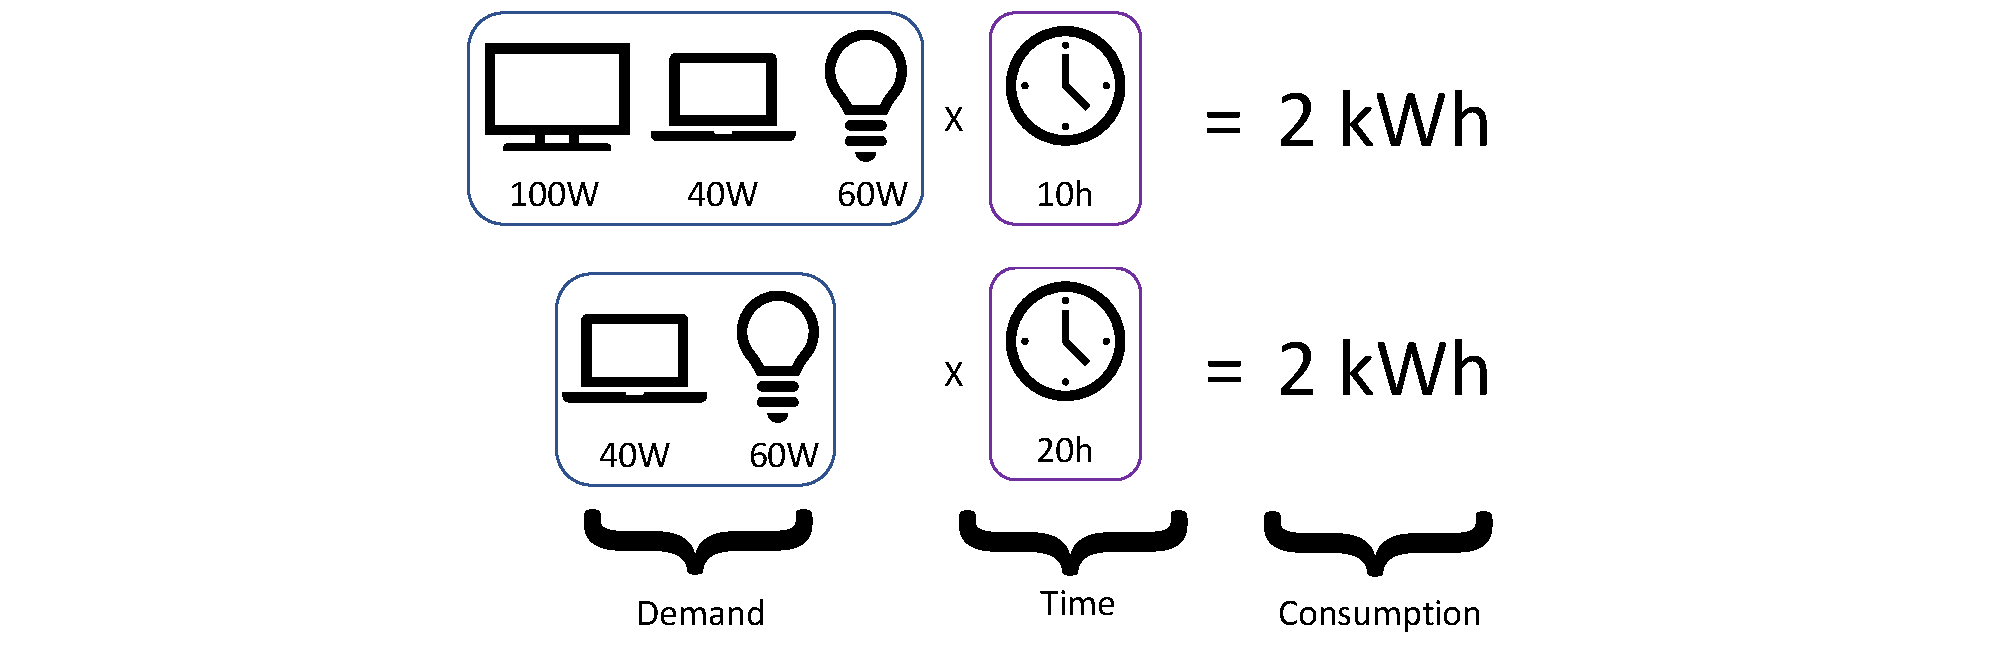
\includegraphics[width=0.80\textwidth]{../figures/DemandConsumption.pdf}
	\caption{Example for demand and consumption}
	\label{fig:demandConsumption}
\end{figure}

The demand is the rate of which we use energy and the consumption is the total energy used for a given time frame \cite{StonyBrookUniversity}. The formulas also show this relation between the consumption and the demand. The consumption is the demand multiplied with the time. If someone turns on 1 heating unit with a demand of 1kW for 2 hours than the demand during this hours is 1kW, but the consumption is 2kWh. The consumption is the same if two heating units are used for half an hour, but the demand is doubled (2kW). Figure \ref{fig:demandConsumption} contains another but similar example. To put it in simple terms the demand is comparable with the speed of a car and the consumption is the distance you drive. The faster you drive the more distance is accumulated over time.